\documentclass[a4paper]{article}

\input ../header
\usepackage{minted}
\usepackage[np]{numprint}
\usepackage{lscape}
\usepackage{afterpage}
\usepackage{hyperref}
\usepackage{gensymb}

\setlength{\multicolsep}{2pt}

% Commandes pour cacher/révéler du texte facilement à l'aide d'un booléen
\usepackage{xstring}
\usepackage{ifthen}

\newboolean{reveal}
\setboolean{reveal}{false}

\newlength{\stextwidth} % une nouvelle longueur

\newcommand\x{6}

\newcommand{\guess}[1]{\ifthenelse{\boolean{reveal}}{{\color{red}#1}}{\settowidth{\stextwidth}{#1}\makebox[\stextwidth]{\dotfill}}}

\newcommand{\guessmath}[1]{\ifthenelse{\boolean{reveal}}{\textcolor{red}{#1}}{\settowidth{\stextwidth}{$#1$}\makebox[1.9\stextwidth]{\dotfill}}}

\newcommand{\guessmathbin}[1]{\ifthenelse{\boolean{reveal}}{\mathbin{\color{red}#1}}{\settowidth{\stextwidth}{$#1$}\makebox[2\stextwidth]{\dotfill}}}

\begin{document}

\title{Chapitre 6 -- Géolocalisation}

\pagestyle{empty}

\date{}
\author{}

\maketitle{}

\thispagestyle{empty}
\noindent\textbf{Activité 2}\hfill{}\textbf{Se repérer sur Terre}
\smallskip
\hrule
\medskip

\begin{multicols}{2}

Tout point sur la surface de la Terre peut être repéré par des coordonnées : sa longitude et sa latitude.

\bigskip

La latitude, souvent notée $\varphi$, est l'angle formé entre la verticale du lieu considéré, et le plan équatorial. Elle est donnée en degré, de $0$\degree{} à $90$\degree{} des deux côtés de l'équateur, en précisant la latitude Nord ou Sud.

\bigskip

La longitude, notée $\lambda$, est l'angle \og{}pointant\fg{} vers l'Ouest ou l'Est par rapport au méridien de Greenwich. La longitude peut être donnée au maximum à $180$\degree{} à l'Est et à $180$\degree{} à l'Ouest.

\bigskip

Un degré est subdivisé en $60$ minutes d'arc (de symbole $'$, \og{}prime\fg{}), elles-mêmes divisées en $60$ secondes d'arc (de symbole $''$, \og{}double prime\fg{}).

\begin{enumerate}
  \item À l'aide du site \url{https://www.coordonnees-gps.fr/}, déterminer la latitude et la longitude de la Tour Eiffel en degrés décimaux.\rep{2}
  \item Donner également ces coordonnées en degrés, minutes et secondes.\rep{2}
  \item Retrouver la réponse de la première question en utilisant Google Maps. Décrire votre démarche.\rep{4}
  \item Que trouve-t-on à environ $17$\degree{} $32'$ $46,748''$ S $149$\degree{} $34'$ $36,964''$ O ? On utilisera Google Maps.\rep{4}
\end{enumerate}

\begin{center}
  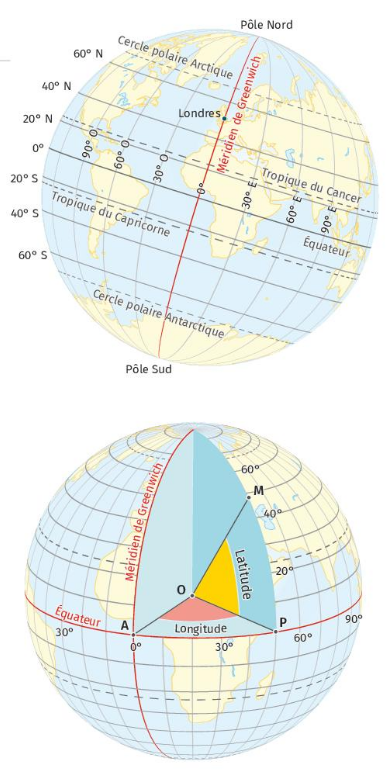
\includegraphics[width=8cm]{latitude_longitude.png}
\end{center}

\end{multicols}

\subsection*{Quelques exercices}

\medskip

\exo \vspace{-2mm}
\begin{multicols}{2}
  \begin{enumerate}
    \item Indiquer du mieux possible les coordonnées géographiques des cinq villes ci-contre.
    \item Colorer :
      \begin{enumerate}
	\item en rouge, tous les points de latitude $23$\degree{} $N$ (tropique du Cancer);
	\item en vert, tous les points de latitude $23$\degree{} $S$ (tropique du Capricorne);
	\item en bleu, tous les points de longitude $10$\degree{} $E$.
      \end{enumerate}
  \end{enumerate}

  \vspace*{0.8cm}
  \begin{center}
    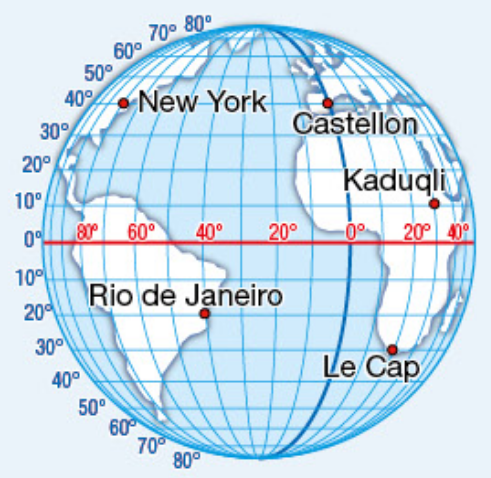
\includegraphics[width=4.5cm]{figure_1.png}
  \end{center}
\end{multicols}

\bigskip

\exo \vspace*{-2mm}
\begin{multicols}{2}
  On a placé sur la sphère terrestre ci-contre différents lieux.
  \begin{enumerate}
    \item Citer deux lieux qui ont la même latitude.
    \item Citer deux lieux qui ont la même longitude.
    \item Quel lieu a pour coordonnées géographiques $30\degree{}N;70\degree{}E$ ?
  \end{enumerate}

  \vspace*{1.5cm}
  \begin{center}
    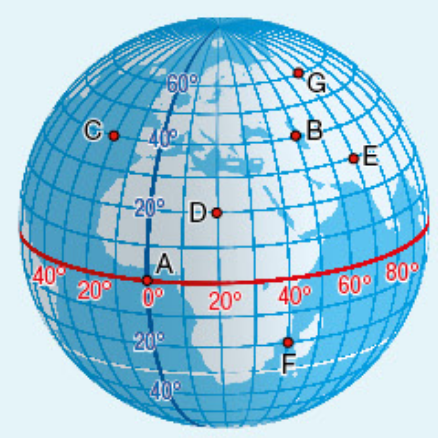
\includegraphics[width=4.5cm]{figure_2.png}
  \end{center} 
\end{multicols}

\bigskip

\exo \vspace*{-2mm}

\begin{multicols}{2}
  La figure ci-contre donne le trajet d'un avion de Morisburg ($D$) aux États-Unis à Kariba ($F$) au Zimbabwe.
  \begin{enumerate}
    \item Donner les coordonnées géographiques du lieu de départ et du lieu d'arrivée.
    \item Déterminer la latitude Nord et la longitude Est les plus élevées atteintes par l'avion.
    \item Existe-t-il une latitude par laquelle l'avion est passé quatre fois ?
  \end{enumerate}

  \vspace*{0.8cm}
  \begin{center}
    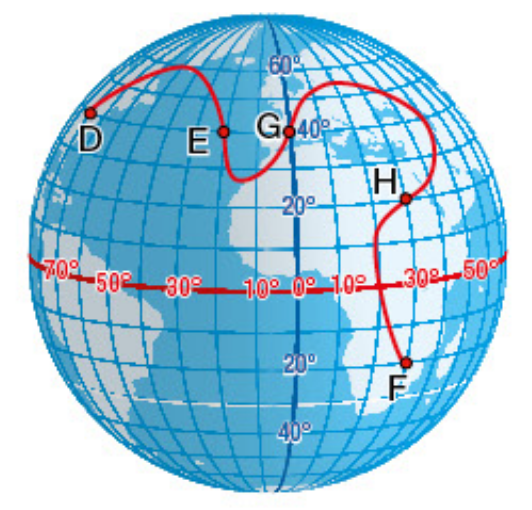
\includegraphics[width=4.7cm]{figure_3.png}
  \end{center}
\end{multicols}

\bigskip

\exo Dans cet exercice, on assimile la Terre à une sphère de rayon $\np{6371}$ kilomètres.
\begin{enumerate}
  \item Déterminer la longueur d'un méridien.
  \item Dunkerque et Barcelone ont pratiquement la même longitude : $2,2$\degree{} Est. La latitude de Dunkerque est de $\np{51,034}$\degree{} Nord et la latitude de Barcelone est de $41,38$\degree{} Nord. En utilisant la proportionnalité de la longueur d'un arc de cercle et de la mesure de l'angle au centre qui l'intercepte, calculer la distance séparant ces deux villes.
\end{enumerate}

\bigskip

\exo \vspace*{-2mm}
On considère un point $A$ situé sur le parallèle de latitude $48$\degree{} Nord que l'on note $\mathcal{C}$. On note $H$ le centre du cercle $\mathcal{C}$ et $O$ le centre de la Terre.

\begin{multicols}{2}
  \begin{enumerate}
    \item
      \begin{enumerate}
	\item Donner une mesure de l'angle $\widehat{AOH}$.
	\item En déduire le rayon du cercle $\mathcal{C}$.
      \end{enumerate}
    \item Les coordonnées géographiques de Quimper (France) sont $(48\degree{}N;4,1\degree{}O)$ et celle de Donetsk (Ukraine) $(48\degree{}N;37,8\degree{}E)$. En utilisant les résultats précédents, estimer la distance parcourue pour rejoindre Donetsk en partant de Quimper et en restant sur le parallèle de latitude $48\degree{}$ Nord.

      \vspace*{1cm}
      \begin{center}
	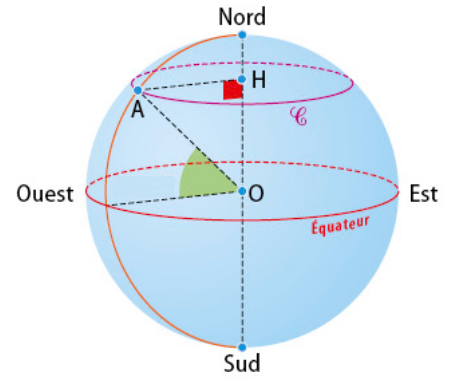
\includegraphics[width=5.5cm]{figure_4.png}
      \end{center}
  \end{enumerate}
\end{multicols}
\end{document}
